\chapter{Prehľad~problematiky}\label{ch:terminology}

Táto kapitola sa zaoberá základnými pojmami a definíciami, ktoré sú nevyhnutné pre pochopenie problematiky tejto práce.

Najskôr sa zameriame na teóriu grafov, ktorá je základom pre analýzu a modelovanie sietí. Definujeme si kľúčové pojmy, ako sú graf,
vrchol, hrana, stupeň a ďalšie. 

Následne sa pozrieme na rôzne typy modelov sietí a ich vlastnosti, predovšetkým na náhodné a
bezškálové siete. Budeme sa sústrediť na ich vznik a charakteristiky, ako je distribúcia stupňov vrcholov.
Taktiež sa budeme venovať slovným sieťam, ktoré sú špecifickým typom sietí, využívaným na analýzu jazyka a
jeho štruktúry.

Na záver kapitoly sa zameriame na úlohu a význam interpunkcie v jazyku a jej vplyvu na štruktúru textu.

\section{Teória~grafov}\label{sec:graph-theory}

Teória grafov je rozsiahla a komplexná oblasť matematiky a informatiky. V tejto kapitole sa zameriame na základné 
pojmy, definície a koncepty, ktoré sú nevyhnutné na pochopenie práce s grafmi, ich vlastností a rôznych aplikácií. 
Pre podrobnejšie informácie a hlbšie pochopenie odporúčam odbornú literatúru, najmä publikáciu
\textit{Graph Theory Fifth Edition od R. Diestela} \cite{diestel2017graph} .

Graf $G$ je reprezentovaný ako dvojica $G = (V, E)$, pričom $V$ \textit{(z angl. vertices)} je množina všetkých
vrcholov a $E$ je množina všetych hrán \textit{(z angl. edges)}, ktoré tvoria spojenia medzi týmito vrcholmi.
Vrcholy grafu sa taktiež nazývajú aj uzly.

Medzi dvojicou vrcholov grafu môže, ale nemusí existovať hrana. Ak medzi nimi hrana existuje, hovoríme, že sú
navzájom prepojené. Jednotlivé hrany, ktoré obsahuje množina $E$, sú reprezentované ako dvojice vrcholov $(u, v)$, 
pričom $u$ a $v$ sú vrcholy z množiny $V$. 

Rozlišujeme niekoľko typov hrán. Ak má hrana grafu daný smer, nazýva sa orientovaná a záleží
na poradí vrcholov v usporiadanej dvojici, prvý vrchol dvojice predstavuje uzol, od ktorého hrana vychádza a 
druhý vrchol dvojice predstavuje uzol, do ktorého hrana smeruje. Ak hrana nemá určený smer, tak sa jedná o 
neorientovanú hranu a poradie vrcholov v usporiadanej dvojici nie je dôležité. Hranu, ktorá má začiatok a koniec 
v rovnakom vrchole, nazývame slučka. Pojem viacnásobná hrana označuje prípad, kedy medzi dvoma vrcholmi existuje viac ako jedna hrana. 
Rôzne typy hrán je možné vidieť na ilustračnom obrázku č. \ref{obr:edges} .

\begin{figure}
    \centerline{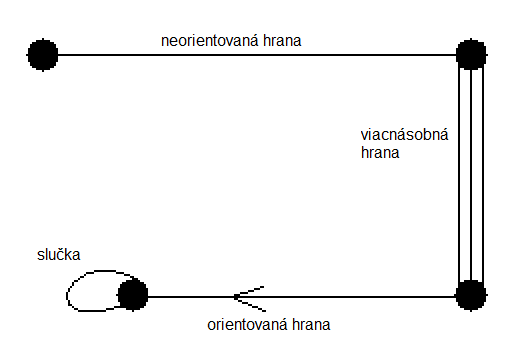
\includegraphics[width=0.5\textwidth]{images/edges.png}}
    \caption[Zobrazenie typov hrán v grafe.]{Zobrazenie typov hrán v grafe.}
    \label{obr:edges}
\end{figure}

Hrany, ktoré majú priradenú číselnú hodnotu, nazývame vážené hrany. Tieto váhy môžu reprezentovať rôzne vlastnosti hrany, 
ako napríklad vzdialenosť medzi vrcholmi alebo náklady na prechod medzi nimi. Sú využívané hlavne v praktických aplikáciách,
ako napríklad dopravné siete.

Pojem jednoduchý graf definuje taký graf, ktorý neobsahuje slučky ani viacnásobné hrany. Jednoduchý graf, ktorý neobsahuje 
orientované hrany a vrcholy sú poprepájané spôsobom každý s každým nazývame kompletný graf \cite{markovsovadynamika} .

Pri analýze grafov je potrebné poznať rôzne spôsoby, akými môžeme prechádzať cez vrcholy a hrany grafu.
Prechod grafom, pri ktorom sa striedajú vrcholy a hrany, ktoré sa môžu opakovať, sa nazýva sled.
Formálny zápis pre sled v grafe $G = (V, E)$ je postupnosť 
\[
v_0, e_0, v_1, e_1, \dots, e_{k-1}, v_{k},
\]
kde $v_i \in V(G)$ pre všetky $i \in \{0, 1, \dots, k\}$ a $e_j \in E(G)$ pre všetky $j \in \{0, 1, \dots, k-1\}$ s podmienkou
$e_i = (v_i, v_{i+1})$. Ťah je špeciálny typ sledu, pri ktorom sa hrany nemôžu opakovať, teda pre všetky $i \neq j$ platí $e_i \neq e_j$.
Vrcholy sa v ťahu môžu opakovať. Sled a ťah majú špeciálny prípad, kedy sa počiatočný a koncový vrchol zhodujú, teda $v_0 = v_k$.
Takýto sled sa nazýva uzavretý sled a ťah uzavretý ťah. Ešte existuje pojem cesta, ktorý predstavuje prechod grafom, pri ktorom sa
nemôžu opakovať ani vrcholy ani hrany.

Spojitý graf je taký graf, v ktorom existuje cesta medzi každými dvoma vrcholmi. Nie každý graf je spojitý, pretože niektoré grafy sa
skladajú z viacerých disjunktných častí, ktoré nie sú navzájom prepojené hranou, teda medzi nimi neexistuje žiadna cesta. Takýmto
disjunktným častiam grafu hovoríme komponenty. Graf s viacerými komponentami je nespojitý graf.

Grafy sa dajú reprezentovať rôznymi spôsobmi. Najčastejšia matematická reprezentácia je pomocou matice susedností a matice incidencie.
Nech $G = (V, E)$ je graf s $n = |V|$ vrcholmi a $m = |E|$ hranami. Matica susedností $A$ je $n \times n$ matica, kde každý prvok $a_{ij}$
predstavuje počet hrán medzi vrcholmi $v_i$ a $u_j$. Incidenčná matica $B$ je $n \times m$ matica, kde pre každý prvok platí $b_{ij} = 1$,
ak je hrana $e_j$ incidentná s vrcholom $v_i$, inak $b_{ij} = 0$.
Príklad matice susedností a incidenčnej matice spolu s ilustračným grafom je zobrazený na obrázku č. \ref{obr:matrices} .

\begin{figure}
    \centerline{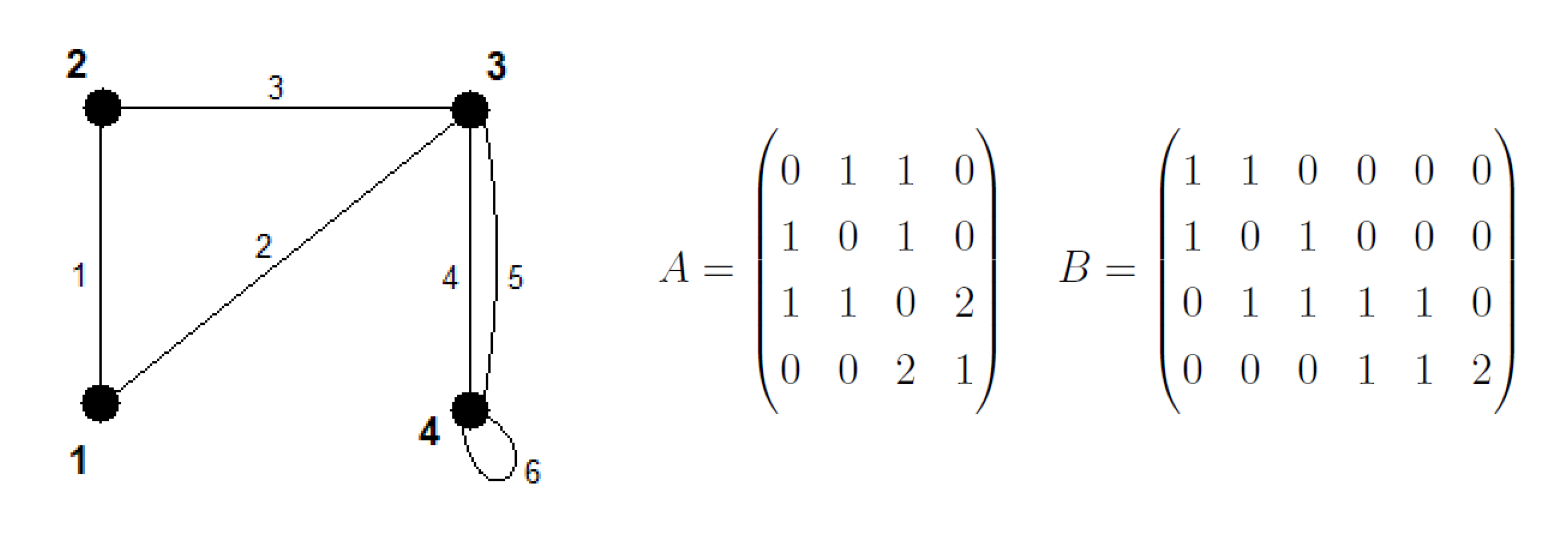
\includegraphics[width=0.8\textwidth]{images/matrices.png}}
    \caption[Matica susedností a incidenčná matica.]{Matica susedností a incidenčná matica pre zobrazený graf.}
    \label{obr:matrices}
\end{figure}

Teraz si predstavíme niekoľko základných vlastností, s ktorými budeme pracovať, ich definície z teórií grafov a ich aplikáciu. Budeme sa zaoberať iba
jednoduchými, neorientovanými grafmi, ak nebude uvedené inak.

Jedna zo základných vlastností vrchola grafu je jeho stupeň. Stupeň vrchola $v$ označovaný aj ako $deg(v)$ nám udáva počet hrán,
ktoré sú incidentné s vrcholom $v$. Minimálna hodnota stupňa vrchola je $0$, vtedy tvorí vrchol samostatný komponent, taktiež sa
nazýva izolovaný vrchol. Maximálna hodnota stupňa vrchola je $n-1$, nastáva keď vrchol susedí s každým vrcholom grafu.
Celkový počet hrán v grafe potom získame ako polovicu súčtu všetkých stupňov vrcholov grafu,
pretože každá hrana je incidentná s dvoma vrcholmi. Tento vzťah môžeme zapísať ako:
\begin{equation}
    |E| = \frac{1}{2} \sum_{i=1}^{n} deg(v_i),
    \label{eq:pocet_hran}
\end{equation}
kde $|E|$ predstavuje počet hrán v grafe a $n$ je počet vrcholov \cite{barabasi2016network} .

Taktiež často používanou charakteristikou grafu je priemerný stupeň uzla:
\begin{equation}
    \bar{d} = \frac{1}{n} \sum_{i=1}^{n} deg(v_i) = \frac{2|E|}{n},
    \label{eq:priemerny_stupen}
\end{equation}
kde $\bar{d}$ je priemerný stupeň uzla a $n$ je počet vrcholov grafu \cite{barabasi2016network} .

Hustota grafu určuje, ako blízko je graf ku kompletnému, teda akú časť z maximálneho počtu hrán obsahuje.
Nadobúda hodnoty v intervale $[0, 1]$, pričom $0$ znamená, že graf je prázdny a $1$ znamená, že graf je kompletný.
Formálny zápis pre hustotu grafu je:
\begin{equation}
    D = \frac{2|E|}{n(n-1)},
    \label{eq:hustota}
\end{equation}
kde $D$ je hustota grafu, $|E|$ je počet hrán a $n$ je počet vrcholov.

Ďalšou vlastnosťou grafu je koeficient zhlukovania, inak známy aj ako klasterizačný koeficient.
Tento koeficient udáva ako veľmi sú prepojené susedné vrcholy uzla. Hodnota koeficientu sa pohybuje v intervale $[0, 1]$,
kde $0$ značí, že medzi susedmi vrcholu neexistujú žiadne hrany a $1$ znamená, že všetci susedia sú medzi sebou navzájom prepojení.
Nech $v$ je vrchol grafu a $deg(v)$ je jeho stupeň, potom:
\begin{equation}
    C_v = \frac{2|E_v|}{deg(v)(deg(v)-1)},
    \label{eq:koeficient_zhlukovania_local}
\end{equation}
kde $C_v$ je koeficient zhlukovania vrchola $v$, $|E_v|$ predstavuje počet hrán medzi $deg(v)$ susedmi vrchola $v$. 
Týmto spôsobom vieme získať lokálny koeficient zhlukovania pre každý vrchol grafu, z ktorých potom vieme vypočítať
priemerný koeficient zhlukovania pre celý graf:
\begin{equation}
    C = \frac{1}{n} \sum_{i=1}^{n} C_{v_i},
    \label{eq:koeficient_zhlukovania_global}
\end{equation}
kde $C$ je priemerný koeficient zhlukovania grafu a $n$ je počet vrcholov grafu \cite{barabasi2016network} .

Pojem najkratšia cesta v grafe definuje takú cestu, ktorá spája dva vrcholy grafu a obsahuje najmenší možný počet
hrán. Priemerná najkratšia cesta medzi dvoma vrcholmi je definovaná ako priemer všetkých najkratších ciest medzi
všetkými kombináciami dvojíc vrcholov grafu.	
\begin{equation}
    \ell = \frac{1}{n(n - 1)} \sum_{\substack{i,j = 1 \\ i \ne j}}^{n} d(v_i, v_j),
    \label{eq:avg_shortest_path}
\end{equation}
kde $\ell$ je priemerná najkratšia cesta, $d(v_i, v_j)$ je dĺžka najkratšej cesty medzi vrcholmi $v_i$ a $v_j$ a $n$ je počet vrcholov grafu \cite{barabasi2016network} .

Priemer grafu udáva najväčšiu dĺžku najkratšej cesty medzi dvoma rôznymi vrcholmi grafu.
\begin{equation}
    diam = \max_{i \ne j} d(v_i, v_j),
    \label{eq:diameter}
\end{equation}

Veľmi dôležitým parametrom pri analýze grafu je distribúcia stupňov vrcholov, značené ako $p_{\mathrm{deg}}$.
Poskytuje pravdepodobnosť, že náhodne vybraný vrchol grafu má práve $\mathrm{deg}$ susedov \cite{barabasi2016network} .
Pre graf s počtom vrcholov $n$ a počtom vrcholov so stupňom $\mathrm{deg}$ označeným ako $n_{\mathrm{deg}}$ je distribúcia stupňov definovaná ako:
\begin{equation}
    p_{\mathrm{deg}} \cong \frac{n_{\mathrm{deg}}}{n},
    \label{eq:degree_distribution}
\end{equation}
kde $p_{\mathrm{deg}}$ predstavuje pravdepodobnosť výskytu daného stupňa, $n_{\mathrm{deg}}$ je počet vrcholov s daným stupňom a $n$ je počet vrcholov grafu.

Najznámejšou a najjednoduchšou mierou centrality je stupňová centralita, ktorá je definovaná ako počet hrán incidentných s vrcholom:
\begin{equation}
    C_D(v) = deg(v),
    \label{eq:degree_centrality}
\end{equation}
kde $C_D(v)$ je stupňová centralita vrchola $v$ a $deg(v)$ je stupeň vrchola $v$ \cite{borgatti2006graph}.

Ďalšou dôležitou centralitou je blízkostná centralita, ktorá hodnotí, ako blízko sa vrchol nachádza k ostatným vrcholom v grafe:
\begin{equation}
    C_C(v) = \frac{|V|-1}{\sum_{\substack{u \in V}} d(v, u)},
    \label{eq:closeness_centrality}
\end{equation}
kde $C_C(v)$ je blízkostná centralita vrchola $v$, $d(v, u)$ je dĺžka najkratšej cesty medzi vrcholmi $v$ a $u$ a $V$
je množina všetkých vrcholov v grafe \cite{borgatti2006graph}.

Významnou centralitou je aj medziľahlosť, ktorá meria, ako často je vrchol súčasťou najkratších ciest medzi inými dvojicami vrcholov:
\begin{equation}
    C_B(v) = \sum_{\substack{u, w \in V \\ u \ne v \ne w}} \frac{\sigma_{uw}(v)}{\sigma_{uw}},
    \label{eq:betweenness_centrality}
\end{equation}
kde $C_B(v)$ je medziľahlosť vrchola $v$, $\sigma_{uw}$ je počet najkratších ciest medzi vrcholmi $u$ a $w$ a $\sigma_{uw}(v)$ je počet týchto ciest,
ktoré prechádzajú cez vrchol $v$ \cite{borgatti2006graph}.


\section{Modely~sietí}\label{sec:network-models}

Siete sú štruktúry, ktoré možno reprezentovať ako grafy skladajúce sa z uzlov (vrcholov) a prepojení (hrán), pričom uzly predstavujú jednotlivé entity
a prepojenia reprezentujú vzťahy medzi nimi. Pojem graf sa používa matematickej reprezentácií, zatiaľ čo termín sieť
často odkazuje na reálne systémy. Umožňujú modelovanie a analýzu komplexných systémov v rôznych odvetviach,
ako informatika, biológia, sociológia a iné \cite{barabasi2016network} . Medzi základné topológie sietí patria náhodné siete a bezškálové siete,
ktoré predstavujú odlišné prístupy ku vzniku a distribúcii prepojení.


\subsection{Náhodná~sieť}\label{sec:random-network}

Náhodná sieť predstavuje jeden zo základných konceptov v teórií sietí. Definujú sa dva základné modely náhodných sietí.

Prvý z nich je Erdős-Rényiho model, $G_{V,H}$, kde $V$ je množina vrcholov a $H$ je množina náhodne vybraných hrán \cite{erdos1959random}\cite{barabasi2016network} .
Tento model generuje náhodnú sieť tak, že začne s $n = |V|$ izolovanými vrcholmi a následne náhodne pridáva $m = |H|$ rôznych hrán medzi nimi,
ktoré sa vyberajú z $\frac{n*(n-1)}{2}$ všetkých možných hrán.

Druhý model je Gilbertov model, $G_{V,p}$, takisto obsahuje $n = |V|$ vrcholov, však hrany nie sú pridelené pevným počtom,
ale nezávisle s pravdepodobnosťou $p$ \cite{gilbert1959random}\cite{barabasi2016network} . Model začína s $n$ izolovanými vrcholmi a následne pre každú dvojicu vrcholov
$u$ a $v$ pridá hranu medzi nimi s pravdepodobnosťou $p$, pričom výsledný počet hrán je náhodný a závisí od hodnoty $p$.

Priemerný stupeň vrchola v náhodnej sieti pre model $G_{V,H}$ vieme vypočítať jednoduchým vzorcom:
\begin{equation}
    \bar{d} = \frac{2|H|}{n},
    \label{eq:avg_degree_random}
\end{equation}
keďže poznáme počet všetkých hrán $|H|$, aj vrcholov n \cite{barabasi2016network} . Pre výpočet priemerného stupňa vrchola
v Gilbertovom modeli $G_{V,p}$ môžeme použiť vzorec \cite{barabasi2016network} :

\begin{equation}
    \bar{d} = \frac{2<L>}{n} = p(n-1),
    \label{eq:avg_degree_gilbert}
\end{equation}

kde $<L>$ definuje súčin pravdepodobnosti $p$ a počtu párov, ktoré sa snažíme spojiť \cite{barabasi2016network} :
\begin{equation}
    <L> = p\frac{n(n-1)}{2}.
    \label{eq:avg_edges_gilbert}
\end{equation}

Na tvorbu náhodných sietí nemáme veľký vplyv, preto nastáva, že niektoré vrcholy majú veľmi vysoký stupeň, 
zatiaľ čo iné majú veľmi nízky stupeň, dokonca aj nulový. Tieto rozdiely je možné pozorovať na distribúcii
stupňov vrcholov $p_k$, ako je vidieť na obrázku č. \ref{obr:randomdegdist} \cite{barabasi2016network} .

Distribúcia stupňov vrcholov v náhodnej sieti sa riadi binomickou distribúciou, ktorá je definovaná ako \cite{barabasi2016network} :
\begin{equation}
    p_{\mathrm{deg}} = \binom{n-1}{\mathrm{deg}} p^{\mathrm{deg}} (1-p)^{n-1-\mathrm{deg}},
    \label{eq:binomial_distribution}        
\end{equation}

pričom tvar binomickej distribúcie je daný počtom vrcholov $n$, počtom hrán $m$ a pravdepodobnosťou $p$.
Distribúcia stupňov vrcholov v náhodnej sieti sa dá priblížiť Poissonovou distribúciou, ak má veľký počet vrcholov,
ktorá je definovaná ako \cite{barabasi2016network} :
\begin{equation}
    p_{\mathrm{deg}} = \frac{\bar{d}^{\mathrm{deg}} e^{-\bar{d}}}{\mathrm{deg}!},
    \label{eq:poisson_distribution}
\end{equation}

$\bar{d}$ je priemerný stupeň vrchola, ktorý je daný vzorcom \ref{eq:avg_degree_gilbert} .

Koeficient zhlukovania v náhodnej sieti je veľmi nízky, pretože väčšina vrcholov je izolovaných a nie sú prepojené.
Vieme ho jednoducho vypočítať ako:
\begin{equation}
    C = p = \frac{\bar{d}}{n},
    \label{eq:clustering_coefficient_random}
\end{equation}

predstavuje pravdepodobnosť, že dva náhodne vybrané vrcholy sú prepojené \cite{barabasi2016network} .

\begin{figure}
    \centerline{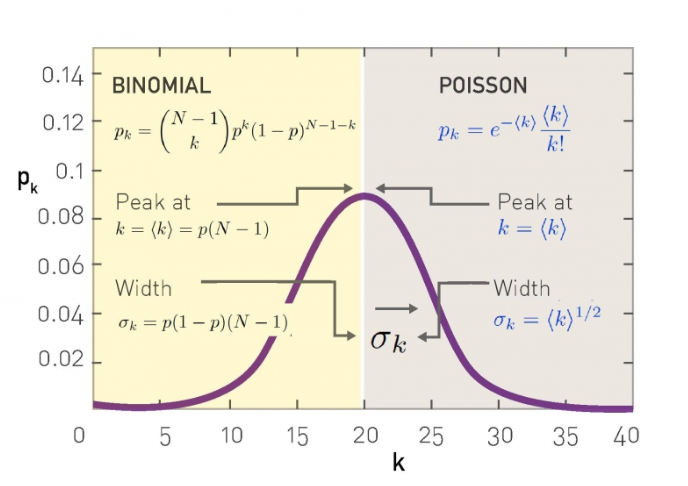
\includegraphics[width=0.8\textwidth]{images/randomdegdist.png}}
    \caption[Binomická vs. Poissonová distribúcia stupňov.]{Binomická vs. Poissonová distribúcia stupňov.
    Presná forma distribúcie náhodnej siete je binomická distribúcia (ľavá strana), pri veľkom počte vrcholov sa
    dá priblížiť Poissonovou distribúciou (pravá strana) \cite{barabasi2016network} .}
    \label{obr:randomdegdist}
\end{figure}

\subsection{Bezškálová~sieť}\label{sec:scale-free-network}

Pri bezškálových sieťach sa jedná o špecifický typ grafu, ktorý sa vyznačuje tým, že existuje niekoľko uzlov
s extrémne vysokým počtom prepojení a väčšina má malý počet prepojení. Tento typ siete sa
v reálnom živote vyskytuje oveľa častejšie ako náhodné siete, najmä v kontextoch ako internet,
biologické siete alebo sociálne siete \cite{barabasi1999emergence} \cite{barabasi2016network} .

Na rozdiel od náhodných sietí, kde sú stupne vrcholov rozdelené podľa binomickej alebo Poissonovej distribúcie, ako je vidno na obrázku č. \ref{obr:randomdegdist} ,
bezškálové siete dodržujú tzv. mocninové rozdelenie (power-law distribution):

\begin{equation}
    p_{\mathrm{deg}} \sim \mathrm{deg}^{-\gamma},
    \label{eq:power_law_distribution_scale_free}
\end{equation}

kde $\gamma$ je škálovací exponent v rozmedzí $2 < \gamma < 3$, ktorý určuje tvar \cite{barabasi2016network} . Pri tomto rozdelení nás najviac zaujíma
rozdelenie stupňov vrcholov, zobrazené v dvojitej logaritimickej mierke, kde produkuje priamku, ako je vidieť na obrázku č. \ref{obr:powerlaw} .

\begin{figure}
    \centerline{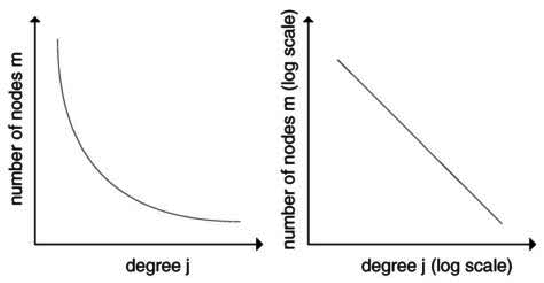
\includegraphics[width=0.8\textwidth]{images/powerlaw.png}}
    \caption[Distribúcia stupňov vrcholov v bezškálovej sieti.]{Distribúcia stupňov vrcholov v bezškálovej sieti \cite{inproceedings} .}
    \label{obr:powerlaw}
\end{figure}

Najznámejší model na generovanie bezškálových sietí je Barabási–Albertov model, označovaný ako $G_{BA}(n, m)$, ktorý má
škálovací exponent $\gamma = 3$. Pri generovaní využíva princíp preferenčného pripájania. Začína s malým počtom počiatočných uzlov a v každom kroku sa pridá nový uzol,
ktorý sa pripojí k $m$ už existujúcim uzlom. Pravdepodobnosť prepojenia nového uzla so starým závisí od stupňa starého uzla \cite{barabasi2016network} :
\begin{equation}
    p(\mathrm{deg(i)}) = \frac{\mathrm{deg(i)}}{\sum_j \mathrm{deg(j)}},
    \label{eq:preferential_attachment}
\end{equation}

Ďalším modelom na generovanie bezškálových sietí je Dorogovtsev–Mendes model, často označovaný ako $G_{DM}(n)$.
Tento model taktiež generuje siete s mocninovým rozdelením stupňov. Od Barabási-Albertovho modelu sa odlišuje mechanizmom rastu siete.
Model začína s trojuholníkom (kompletným grafom s tromi uzlami) a v každom kroku sa pridá nový uzol, ktorý sa pripojí na oba koncové body
náhodne vybranej existujúcej hrany \cite{dorogovtsev2002evolution}. Takýmto spôsobom sa v každom kroku vytvorí nový trojuholník, čo vedie k
vysokému koeficientu zhlukovania. Model teda zabezpečuje vznik sietí, ktoré sú nielen bezškálové, ale majú aj malé
priemerné vzdialenosti medzi uzlami a vysokú mieru zhlukovania.

Zvýšený koeficient zhlukovania sa vyskytuje najmä pri analýze slovných sietí, kde sa rovnaké slová často vyskytujú v blízkosti seba a vytvárajú frázy,
prirodzene sa zhlukujú do skupín. Práve preto je Dorogovtsev-Mendes model vhodný na analýzu jazykových dát, keďže dokáže simulovať podobné vlastnosti, štruktúru
ako majú slovné siete vytvorené na reálnych jazykových dátach. 

\section{Slovné~siete}\label{sec:word-networks}

Slovné siete predstavujú efektívny spôsob reprezentácie a analýzy jazyka a jeho štruktúry za pomoci teórie grafov.
V takýchto sieťach sú jednotlivé slová reprezentované ako uzly a vzťahy medzi slovami, ktoré sa navzájom ovplyvňujú alebo súvisia
tvoria hrany \cite{motter2002topology} . Podľa metód reprezentácie vzťahov medzi slovami dokážeme slovné siete rozlišovať.
V sémantických slovných sieťach vznikajú prepojenia medzi slovami na základe ich významovej podobnosti. Narozdiel od sémantických
slovných sietí, v syntaktických slovných sieťach sú interakcie medzi slovami založené na slovnej štruktúre a gramatických pravidlách.

\pagebreak

Špecifický typ syntaktickej slovnej siete, ktorej sa budeme venovať v tejto práci sa nazýva pozičná slovná sieť. Táto sieť je zameraná na štruktúru
a pozície slov v texte. V pozičnej slovnej sieti uzly tvoria jednotlivé slová a hrany sú vytvorené na základe toho, či sa slová nachádzajú
vedľa seba v texte. Ukážku takejto siete vidíme na obrázku č. \ref{obr:wan} .

Tieto siete majú niekoľko zaujímavých vlastností. Koeficient zhlukovania, ktorý určuje, do akej
miery slová tvoria skupiny alebo často používané frázy. Distribúcia stupňov uzlov je
typu mocninného zákona, čo znamená, že väčšina slov má veľmi nízky stupeň, zatiaľ čo malý podiel slov má veľmi vysoký stupeň \cite{dorogovtsev2001language} .
Toto rozdelenie je typické pre bezškálové siete. Na obrázku č. \ref{obr:degdist} je zobrazená distribúcia stupňov uzlov s dvomi
rôznymi priemernými exponentami $y = -1.5$ a $y = -2.7$. Exponent $y = -2.7$ sa blíži k exponentu pre Barabási-Albertov model, ktorý je
$y_{BA} = -3$ \cite{cancho2001small} .

\begin{figure}
    \centerline{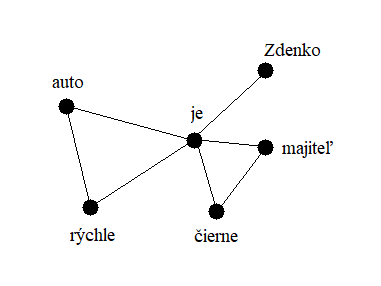
\includegraphics[width=0.8\textwidth]{images/wan.png}}
    \caption[Pozičná slovná sieť.]{Pozičná slovná sieť z viet: „Auto je rýchle. Auto je čierne. Majiteľ je Zdenko.“.}
    \label{obr:wan}
\end{figure}

\begin{figure}
    \centerline{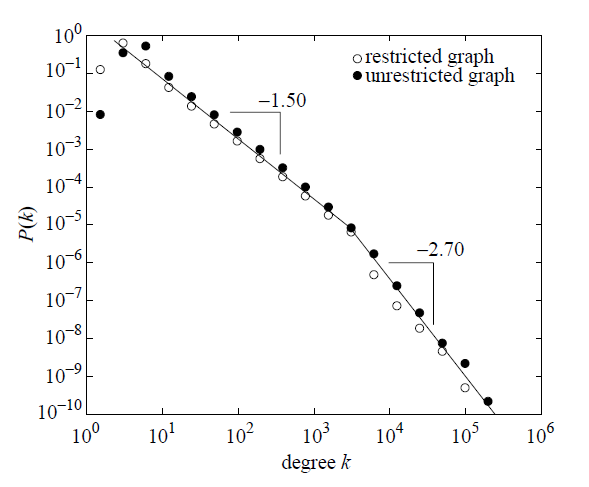
\includegraphics[width=0.8\textwidth]{images/degdist.png}}
    \caption[Distribúcia stupňov vrcholov, Dorogovtsev Mendes model]{Dorogovtsev Mendes model, distribúcia stupňov vrcholov pre dve siete,
    body zoskupené mocninou dvoch \cite{cancho2001small} .}
    \label{obr:degdist}
\end{figure}

\clearpage

\section{Interpunkcia}\label{sec:punctuation}

Interpunkcia je základný prvok jazyka, používa sa na štruktúrovanie a organizovanie textu, vyjadrenie významových vzťahov.
Pri správnom použití interpunkcia zlepšuje čitateľnosť a porozumenie textu, zatiaľ čo nesprávne použitie môže viesť k
nejednoznačnosti a nedorozumeniu \cite{lubis2025mastering}.

Tvorí ju súbor znakov, kde každý znak má svoj osobitý význam a funkciu, ako napríklad pauza, dôraz, ukončenie vety, vzťahy medzi vetnými členmi
a podobne. Pravidlá písania interpunkcie sú kodifikované v gramatických a jazykových príručkách. Taktiež sa pravidlá písania interpunkcie líšia
v závislosti od jazyka, v ktorom je text napísaný.

Najbežnejšie používané interpunkčné znamienka možno rozdeliť do niekoľkých skupín podľa ich funkcie:
ukončovacie (bodka, otáznik, výkričník), oddeľovacie (čiarka, bodkočiarka, dvojbodka), typografické (úvodzovky, zátvorky, pomlčky),
prípadne aj iné znaky (trojbodka, lomka, atď.).

Z gramatického hľadiska interpunkcia rozdeľuje text, vyznačuje vetnú štruktúru, oddeľuje vetné členy, hlavné a vedľajšie vety.
Napríklad umiestnenie čiarky pred spojkami často naznačuje, že ide o vedľajšiu vetu, zatiaľ čo bodka, otáznik, výkričník označujú koniec vetného celku.

Z fonetického hľadiska interpunkcia určuje intonáciu, pauzy pri čítaní textu, dôraz, rytmus a tón. Napríklad bodka naznačuje koniec vety a vyžaduje prestávku,
kým čiarka naznačuje, že čitateľ by mal pokračovať v čítaní s malou pauzou. Takýmto spôsobom interpunkcia dokáže preniesť aspekty reči do písaného textu,
čo môže ovplyvniť jeho význam a interpretáciu.

Zo štylistického hľadiska interpunkcia ovplyvňuje štýl a tón textu. Napríklad použitie výkričníka môže naznačovať dôraz, vážnosť alebo nadšenie, zatiaľ čo otáznik
môže naznačovať pochybnosť. Taktiež môže ovplyvniť rytmus a plynulosť textu. Napríklad dlhé vety s množstvom čiarkami môžu spôsobiť, že text bude pôsobiť ťažkopádne
a zložito, zatiaľ čo krátke vety s minimálnym použitím interpunkcie môžu pôsobiť rýchlo a dynamicky. 